\documentclass[11pt]{article}
\usepackage{amsmath, amsfonts, amsthm, amssymb}  % Some math symbols
\usepackage{fullpage}

\usepackage[x11names, rgb]{xcolor}
\usepackage{graphicx}
\usepackage{tikz}
\usetikzlibrary{decorations,arrows,shapes}

\usepackage{etoolbox}
\usepackage{enumerate}
\usepackage{listings}

\setlength{\parindent}{0pt}
\setlength{\parskip}{5pt plus 1pt}

\newcommand{\N}{\mathbb N}
\newcommand{\E}{\mathbb E}
\newcommand{\V}{Var}
\renewcommand{\P}{\mathbb P}
\newcommand{\f}{\frac}


\newcommand{\nopagenumbers}{
    \pagestyle{empty}
}

\def\indented#1{\list{}{}\item[]}
\let\indented=\endlist

\providetoggle{questionnumbers}
\settoggle{questionnumbers}{true}
\newcommand{\noquestionnumbers}{
    \settoggle{questionnumbers}{false}
}

\newcounter{questionCounter}
\newenvironment{question}[2][\arabic{questionCounter}]{%
    \addtocounter{questionCounter}{1}%
    \setcounter{partCounter}{0}%
    \vspace{.25in} \hrule \vspace{0.4em}%
        \noindent{\bf \iftoggle{questionnumbers}{#1: }{}#2}%
    \vspace{0.8em} \hrule \vspace{.10in}%
}{$ $\newpage}

\newcounter{partCounter}[questionCounter]
\renewenvironment{part}[1][\alph{partCounter}]{%
    \addtocounter{partCounter}{1}%
    \vspace{.10in}%
    \begin{indented}%
       {\bf (#1)} %
}{\end{indented}}

\def\show#1{\ifdefempty{#1}{}{#1\\}}

\newcommand{\header}{%
\begin{center}
    {\Large \show\myhwname}
    \show\myname
    \show\myemail
    \show\mysection
    \today
\end{center}}

\usepackage{hyperref} % for hyperlinks
\hypersetup{
    colorlinks=true,
    linkcolor=blue,
    filecolor=magenta,      
    urlcolor=blue,
}

\newcommand{\myhwname}{Hello}
\newcommand{\myname}{Test}
\newcommand{\myemail}{}
\newcommand{\mysection}{Se}

\noquestionnumbers
\nopagenumbers

%% Redefine overline to ol
\def\ol{\overline}

% Use images
\usepackage{graphicx}

%%%%%%%%%%%%%%%%%% Begin the Document %%%%%%%%%%%%%%%%%%%%%

\begin{document}
%\header
\begin{flushleft}
CSE 312\\
HW 3
\end{flushleft}

%--------------- Problem 1 ---------------%
\begin{question}{Problem 1}

% Problem 1a
\begin{part}

\textbf{Answer:} \fbox{$P(S) = \frac{|\text{Combinations with Ten of Spades in the stock}|}{|\text{Possible combinations of the stock}|} = \frac{\frac{1!}{1!(1-1)!} * \frac{7!}{2!(7-2)!}}{\frac{8!}{3!(8-3)!}} = \frac{3}{8} = 0.375$}

\textbf{Explanation:} 
There are $\frac{8!}{3!(8-3)!} = 56$ ways to choose 3 cards out of 8 for the stock. There is $\frac{1!}{1!(1-1)!} = 1$ way to have the Ten of Spades in the stock. There are $\frac{7!}{2!(7-2)!} = 21$ ways to choose the remaining 2 cards in the stock. The probability of having the Ten of Spades in the stock then is $\frac{1 * 21}{56} = \frac{3}{8} = 0.375$. 
\end{part}

% Problem 1b
\begin{part}

\textbf{Answer:} \fbox{$\text{Minimum points to win} = 66 - (46 + 7) = 13$}

\textbf{Explanation:} 
There are $4 + 10 + 10 + 11 + 11 = 46$ points in your hand. You have $7$ points in tricks. Assuming you are going to win the remaining tricks you already have $46 + 7 = 53$ points. Therefore you need the opponent to have $66 - 53 = 13$ points in their hand to win. 
\end{part}

% Problem 1c
\begin{part}

\textbf{Answer:} \fbox{$P(W | S) = \frac{|W \cap S|}{|S|} = \frac{\frac{7!}{5!(7-5)!} - (\frac{3!}{3!(3-3)!} * \frac{3!}{2!(3-2)!})}{\frac{7!}{5!(7-5)!}} = \frac{6}{7} \approx 0.857$}

\textbf{Explanation:} 
$P(W | S) = \frac{|W \cap S|}{|S|}$. Use method of complements to find the opponent's hands you need to win. There are $\frac{7!}{5!(7-5)!} = 21$ total ways to draw a hand. The only hand that will cause you to lose is one with 3 Jacks and 2 Queens. There is $\frac{3!}{3!(3-3)!} = 1$ way to choose 3 Jacks out of 3 and $\frac{3!}{2!(3-2)!} = 3$ ways to choose 2 Queens out of 3. Therefore, the probability of winning given that the Ten is in the stock is $\frac{21 - (1 * 3)}{21} = \frac{6}{7} \approx 0.8571428571$. 
\end{part}

% Problem 1d
\begin{part}

\textbf{Answer:} \fbox{$\text{Points to win with Ten of Spades not in the stock} = 66 - (10 + 10 + 11 + 11 ) = 17$}

\textbf{Explanation:} 
He will have the Ten of Spades in his hand leaving you 4 cards to take in trick points. If you do not score 66 before he plays Ten of Spades as his last trick, you will lose. You will play your King last so you cannot count it's value among the points you will score leaving you with $10 + 10 + 11 + 11 = 42$ points in your hand and $7$ in tricks for $49$ points total. Therefore, to win by the fourth trick you need your opponent to have $66 - 49 = 17$ points distributed among their 4 non-Ten cards. 
\end{part}

% Problem e
\begin{part}

\textbf{Answer:} \fbox{$P(W \mid \ol{S}) = \frac{|\text{Combinations winning hands with Ten in hand}|}{|\text{Total Combinations of hands with Ten in hand}|} = \frac{\frac{1!}{1!(1-1)!} * \frac{6!}{3!(6-3)!}}{\frac{7!}{4!(7-4)!}} = \frac{4}{7} \approx 0.571$}

\textbf{Explanation:} 
Given the 10 of Spades is not in the stock, then it is in your opponents hand. There are 4 cards left for them to hold. For you to win they must have 17 points in their hand. Without the Ace their highest hand is three Queens and two Jacks which only total fifteen points. With the Ace, their lowest hand is 1 Ace and 3 Jacks totaling 17 points. Therefore, they must hold the Ace for you to win. There is $\frac{1!}{1!(1-1)!} = 1$ way to hold the Ace and $\frac{6!}{3!(6-3)!} = 20$ ways to have a hand composed of 3 Queens and 3 Jacks, any of which will meet the minimum of 17 points required for you to win. There are $\frac{7!}{4!(7-4)!} = 35$ possible hands when the Ten is not in the stock.  Therefore, the probability of winning the hand with the Ten not in the stock is $\frac{1 * 20}{35} = \frac{4}{7} \approx 0.5714285714$. 
\end{part}

% Problem 1f
\begin{part}

\textbf{Answer:} \fbox{$P(W) = P(W \mid S)P(S) + P(W \mid \ol{S})P(\ol{S}) = (\frac{6}{7})(\frac{3}{8}) + (\frac{4}{7})(1 - \frac{3}{8}) = \frac{19}{28} \approx 0.679$}

\textbf{Explanation:} 
Your total probablity of winning is the total probability of hands with and without the Ten of Spades in the stock or $P(W \mid S)P(S) + P(W \mid \ol{S})P(\ol{S})$. The probability therefore of winning the hand is $(\frac{6}{7})(\frac{3}{8}) + (\frac{4}{7})(1 - \frac{3}{8}) = \frac{19}{28} \approx 0.6785714286$ 
\end{part}

\end{question}

%--------------- Problem 2 ---------------%
\begin{question}{Problem 2}

% Problem 2a
\begin{part}

\textbf{Answer:} \fbox{$L_1 = \frac{11}{25} = 0.44, L_2 = \frac{11}{25} = 0.44$}

\textbf{Explanation:}
The probability of choosing a lavender ball on the first draw from the chosen pocket will be it's total probability given whether or not it's drawn on draw D, i.e. $P(L_1) = P(L_1 | D)P(D) + P(L_1 | \ol{D})P(\ol{D})$. This works out to $(\frac{3}{5})(\frac{3}{5}) + (\frac{1}{5})(\frac{2}{5}) = \frac{11}{25} =  0.44$. Because the chosen pocket is not changed after the first draw from it and any ball removed from it is returned, the probabilty of $L_2$ is the same as $L_1$, i.e. $\frac{11}{25} = 0.44$. 
\end{part}

% Problem 2b
\begin{part}

\textbf{Answer:} \fbox{$P(L_2 \mid L_1) = \frac{P(L_1 \cap L_2)}{P(L_1)} = \frac{\frac{3}{5} * \frac{3}{5} * \frac{3}{5} + \frac{2}{5} * \frac{1}{5} * \frac{1}{5}}{\frac{11}{25}} = \frac{29}{55} \approx 0.527$}

\textbf{Explanation:}  
The probability of choosing $L_2$ given $L_1$ is $\frac{P(L_1 \cap L_2)}{P(L_1)}$. By part (c) we know that $L_1$ and $L_2$ are dependent. The probability of the intersection of $L_1$ and $L_2$ is the total probability $\frac{3}{5} * \frac{3}{5} * \frac{3}{5} + \frac{2}{5} * \frac{1}{5} * \frac{1}{5} = \frac{29}{125} = 0.232$. From part (a) the probability of $L_1$ is $\frac{11}{25} = 0.44$. So the probability of $L_2$ given $L_1$ is $\frac{\frac{29}{125}}{\frac{11}{25}} = \frac{29}{55} \approx 0.5272727273$. 
\end{part}

% Problem 2c
\begin{part}

\textbf{Answer:} \fbox{No, they're dependent.}

\textbf{Explanation:}
$L_1$ and $L_2$ are independent if and only if $P(L_1 \cap L_2) = P(L_1)P(L_2)$. The probability of intersection of $L_1$ and $L_2$ is known from part (b) to be $\frac{29}{125} = 0.232$. The product of $L_1$ and $L_2$ is $\frac{3}{5} * \frac{3}{5} = \frac{9}{25}$. Because $\frac{29}{125} \neq \frac{9}{25}$, $L_1$ and $L_2$ are not independent. 
\end{part}

% Problem 2d
\begin{part}

\textbf{Answer:} \fbox{$P(D | L_1 \cap L_2) = \frac{P(L_1 \cap L_2 | D)P(D)}{L_1 \cap L_2} = \frac{\frac{9}{25} * \frac{3}{5}}{\frac{29}{125}} = \frac{27}{29} \approx 0.931$}

\textbf{Explanation:}  
The probability of $L_1$ and $L_2$ given $D$ will just be $\frac{3}{5} * \frac{3}{5} = \frac{9}{25}$. $P(D)$ is known to be simply $\frac{3}{5}$. And from part (b) the probability of $L_1 \cap L_2$ is $\frac{29}{125} = 0.232$. So, $P(D | L_1 \cap L_2) = \frac{\frac{9}{25} * \frac{3}{5}}{\frac{29}{125}} = \frac{27}{29} \approx 0.9310344828$. 
\end{part}

\end{question}

%--------------- Problem 3 ---------------%
\begin{question}{Problem 3}

% Problem 3a
\begin{part}

\textbf{Answer:} \fbox{$P(H | \ol{T}) = \frac{P(\ol{T} \mid H)P(H)}{P(\ol{T} \mid H)P(H) + P(\ol{T} \mid \ol{H})P(\ol{H})} = \frac{(0.04)(0.005)}{(0.04)(0.005) + (0.88)(0.995)} = \frac{1}{4379} \approx 2.3 * 10^{-4}$}

\textbf{Explanation:} 
Let H be the event of having the disorder and T the event of the test coming back positive. Apply the corollary of Bayes' Theorem, $P(H | \ol{T}) = \frac{P(\ol{T} \mid H)P(H)}{P(\ol{T} \mid H)P(H) + P(\ol{T} \mid \ol{H})P(\ol{H})}$. Take $P(\ol{T} \mid \ol{H})$ to be the complement of the false positive, i.e. $1 - 0.12 = 0.88$. The remaining percentages are known. Substituting yields $P(H | \ol{T}) = \frac{(0.04)(0.005)}{(0.04)(0.005) + (0.88)(0.995)} = \frac{1}{4379} \approx 0.0002283626399$. One could rest in believing that they probably don't have the disorder 

\end{part}

% Problem 3b
\begin{part}

\textbf{Answer:} \fbox{$P(H | T) = \frac{P(T \mid H)P(H)}{P(T \mid H)P(H) + P(T \mid \ol{H})P(\ol{H})} = \frac{(0.96)(0.005)}{(0.96)(0.005) + (0.12)(0.995)} = \frac{1}{207} \approx 3.9 * 10^{-2}$}

\textbf{Explanation:} 
Apply the corollary of Bayes' Theorem, $P(H | T) = \frac{P(T \mid H)P(H)}{P(T \mid H)P(H) + P(T \mid \ol{H})P(\ol{H})}$. Take $P(\ol{T} \mid \ol{H})$ to be the complement of the false negative, i.e. $1 - 0.04 = 0.96$. The remaining percentages are known. Substituting yields $P(H | \ol{T}) = \frac{(0.96)(0.005)}{(0.96)(0.005) + (0.12)(0.995)} = \frac{1}{207} \approx 0.038647343$. The test doesn't seem very reliable. 
\end{part}

% Problem 3c
\begin{part}

\textbf{Answer:} \fbox{$P(H | \ol{T}) = \frac{P(\ol{T} \mid H)P(H)}{P(\ol{T} \mid H)P(H) + P(\ol{T} \mid \ol{H})P(\ol{H})} = \frac{(0.04)(0.15)}{(0.04)(0.15) + (0.88)(0.85)} = \frac{3}{377} \approx 8.0 * 10^{-3}$}

\textbf{Explanation:}
Apply the corollary of Bayes' Theorem, $P(H | \ol{T}) = \frac{P(\ol{T} \mid H)P(H)}{P(\ol{T} \mid H)P(H) + P(\ol{T} \mid \ol{H})P(\ol{H})}$. Take $P(\ol{T} \mid \ol{H})$ to be the complement of the false positive, i.e. $1 - 0.12 = 0.88$. The remaining percentages are known. Substituting yields $P(H | \ol{T}) = \frac{(0.04)(0.15)}{(0.04)(0.15) + (0.88)(0.85)} = \frac{3}{377} \approx 0.007957559682$. 
One can still rest in believing that they probably don't have the disorder given a negative result. 
\end{part}

% Problem 3d
\begin{part}

\textbf{Answer:} \fbox{$P(H | T) = \frac{P(T \mid H)P(H)}{P(T \mid H)P(H) + P(T \mid \ol{H})P(\ol{H})} = \frac{(0.96)(0.15)}{(0.96)(0.15) + (0.12)(0.85)} = \frac{24}{41} \approx 5.9 * 10^{-1}$}

\textbf{Explanation:}  
Apply the corollary of Bayes' Theorem, $P(H | T) = \frac{P(T \mid H)P(H)}{P(T \mid H)P(H) + P(T \mid \ol{H})P(\ol{H})}$. Take $P(\ol{T} \mid \ol{H})$ to be the complement of the false negative, i.e. $1 - 0.04 = 0.96$. The remaining percentages are known. Substituting yields $P(H | \ol{T}) = \frac{(0.96)(0.15)}{(0.96)(0.15) + (0.12)(0.85)} = \frac{24}{41} \approx 0.5853658537$. One should probably have further tests if it's this likely that they have the disorder given a positive result. 
\end{part}

\end{question}

%--------------- Problem 4 ---------------%
\begin{question}{Problem 4}

% Problem 4

\textbf{Answer:} \fbox{$\frac{9}{10}$}

\textbf{Explanation:} 
We solve for $p_0$ but that leaves us with $p_1$ and $p_{-1}$ undefined. We have to then solve for those. Because the game ends at $+2$ and $-2$ points, when we have $p_2$ and $p_{-2}$ we can directly change those to the probability of winning or losing, $1$ and $0$, respectively. Plugging in $p_1$ and $p_{-1}$ to $p_0$ we can replace those in the $p_0$ equation. Finally, we can plug in $P(S) = \frac{3}{4}$ and solve. 
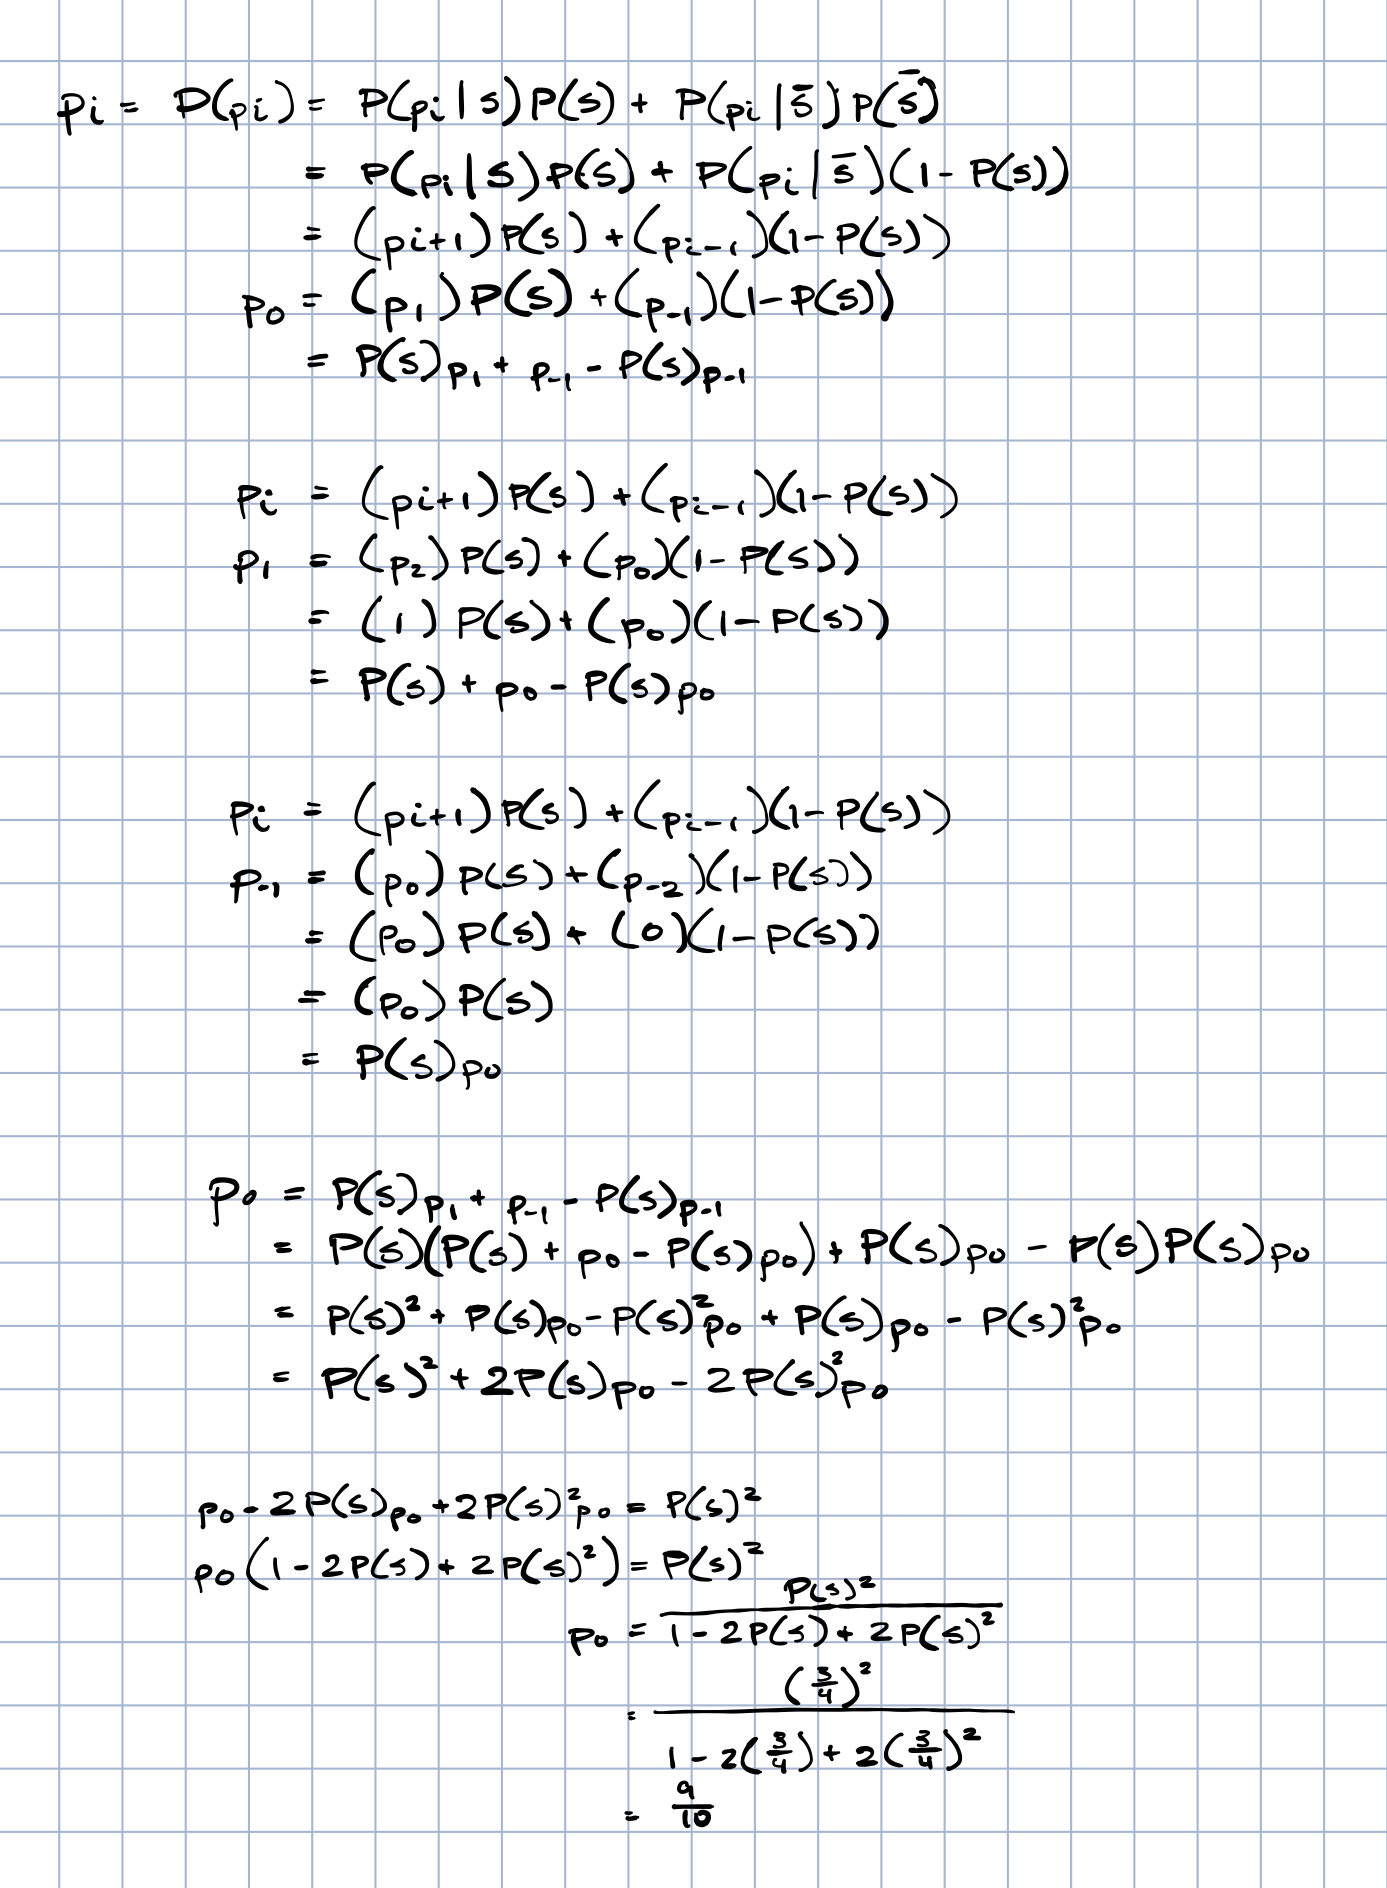
\includegraphics[scale=0.4]{hw3p7a}

\end{question}

%--------------- Problem 5 ---------------%
\begin{question}{Problem 5}

% Problem 5a
\begin{part}

\textbf{Answer:} \fbox{$P(\text{Apple carries O} \mid \text{Apple has type A}) = \frac{P(\text{Apple carries O})}{P(\text{Apple has type A})} = \frac{\frac{2}{4}}{\frac{3}{4}} = \frac{2}{3} \approx 0.667$} 

\textbf{Explanation:} 
The only possible arrangement of the parent's blood types such that they both have Type A, Apple has type A, and Olive has type O, is for both of them to have $\{A,O\}$. From this, there is a $\frac{3}{4} = 0.75$ probability of Apple having type A. Given that Apple has Type A, 2 of those possibilities have an O gene, or she has a $\frac{2}{4} = 0.5$ probability of having an O gene. Therefore, her probability of having an O gene given that she has type A blood is $\frac{\frac{2}{4}}{\frac{3}{4}} = \frac{2}{3} \approx 0.6666666667$. 
\end{part}

% Problem 5b
\begin{part}

\textbf{Answer:} \fbox{$P(\text{First child has type O}) = \frac{1}{3} * 0 + \frac{2}{3} * \frac{2}{4} = \frac{1}{3} \approx 0.3333333333$}

\textbf{Explanation:}  
The probability of Apple and Oscar's first child having type O is the total probabilty of the events. There are two possible ways Apple could have type A, $\{A,A\}$ and $\{A,O\}$ with a probability of $\frac{1}{3}$ and $\frac{2}{3}$, respectively. The probabilty of child one having O in the first case is $0$ and $\frac{2}{4} = 0.5$ in the second. Therefore, the probability of the first child having type O blood is $\frac{1}{3} * 0 + \frac{2}{3} * \frac{2}{4} = \frac{1}{3} \approx 0.3333333333$. 
\end{part}

% Problem 5c
\begin{part}

\textbf{Answer:} \fbox{$\frac{P(\text{First child has type A} \mid \text{Apple carries O})P(\text{Apple carries O})}{P(\text{First child has type A})} = \frac{\frac{1}{2} * \frac{2}{3}}{\frac{2}{3}} = \frac{1}{2} = 0.5$}

\textbf{Explanation:}
The probability of Apple carrying an O gene in this case is found by Bayes Theorem. The probability of the first child having type A given that Apple carries an O gene is $\frac{2}{4} = \frac{1}{2} = 0.5$. The probability of Apple having type A is known to be $\frac{2}{3}$ from part (a) and the probabilty of the first child having type A is the complement of it having type O or $1 - \frac{1}{3} = \frac{2}{3} = approx 0.6666666667$. Therefore, the probabiltity of Apple carrying an O gene given her first child carries an A gene is $\frac{\frac{1}{2} * \frac{2}{3}}{\frac{2}{3}} = \frac{1}{2} = 0.5$. 
\end{part}

% Problem 5d
\begin{part}

\textbf{Answer:} \fbox{$\frac{P(C_1)P(C_2)P(A_{AO}) + P(C_1)P(C_2)P(A_{AA})}{P(C_1)} = \frac{(\frac{2}{3})(\frac{1}{3})(\frac{1}{3}) + (1)(1)(\frac{1}{3})}{\frac{2}{3}} = \frac{3}{4} = 0.75$}

\textbf{Explanation:}
The total probability of Child 1 and Child 2 having type A is $P(C_1)P(C_2)P(A_{AO}) + P(C_1)P(C_2)P(A_{AA}) = (\frac{2}{3})(\frac{1}{3})(\frac{1}{3}) + (1)(1)(\frac{1}{3}) = \frac{1}{2}$. This, divided by the probability of $P(C_1) = \frac{2}{3}$ having type A is $\frac{(\frac{2}{3})(\frac{1}{3})(\frac{1}{3}) + (1)(1)(\frac{1}{3}) = \frac{1}{2}}{\frac{2}{3}} = \frac{3}{4} = 0.75$. 
\end{part}

% Problem 5e
\begin{part}

\textbf{Answer:} \fbox{No, they're dependent.}

\textbf{Explanation:}
$C_1$ and $C_2$ are independent if and only if $P(C_2 \mid C_1) = P(C_2)$. $P(C_2 \mid C_1) = \frac{3}{4}$ from part (d) but $P(C_2) = \frac{2}{3}$. Because they are not equal, the blood types of the children are dependent. 
\end{part}

\end{question}

%--------------- Problem 6 ---------------%
\begin{question}{Problem 6}

% Problem 6a
\begin{part}

\textbf{Answer:} \fbox{${n \choose k} p^k (1 - p)^{n - k} = {8 \choose 2} 0.258^{2} (1 - 0.258)^{8 - 2} \approx 3.11 * 10^{-1}$}

\textbf{Explanation:} 
The probability of no trumps in exactly 2 hands out of 8 can be found using the formula ${n \choose k} p^k (1 - p)^{n - k}$. So, plugging in the values we have for n, p, and k yields ${8 \choose 2} 0.258^{2} (1 - 0.258)^{8 - 2} \approx 0.31104331722062273$. 
\end{part}

% Problem 6b
\begin{part}

\textbf{Answer:} \fbox{$1 - ({8 \choose 0} 0.258^{0} (1 - 0.258)^{8 - 0} + {8 \choose 1} 0.258^{1} (1 - 0.258)^{8 - 1}) \approx 6.53 * 10^{-1}$}

\textbf{Explanation:} 
We want to find the probability of no trumps in 2 or more of the 8 hands, this can be found by taking the complement of no trumps in 0 or 1 hands. So the complement of the sum of the formula from above yields $1 - ({8 \choose 0} 0.258^{0} (1 - 0.258)^{8 - 0} + {8 \choose 1} 0.258^{1} (1 - 0.258)^{8 - 1}) \approx 0.6525318486688256$. 
\end{part}

\end{question}

%--------------- Problem 7 ---------------%
\begin{question}{Problem 7}

% Problem 7a
\begin{part}
\textbf{Answer:} \fbox{$AB = 1 - [(1 - 0.75 * 0.9) * (1 - 0.7 * 0.95)] * 0.85 = 7.5745625 * 10^{-1}$}

\textbf{Explanation:}
We can break this network into components to simplify calculations. Let $AC_{upper}$ be the upper path from A to C and $AC_{lower}$ be the lower path. The probablity of $AC_{upper}$ is $P_1 * P_2$ and $AC_{lower}$ is $P_3 * P_4$. Let AC be the complete path from A to C which can be found by the complement of the product of the probability of failure $AC_{upper}$ and $AC_{lower}$, i.e. $AC = 1 - [(1 - AC_{upper}) * (1 = AC_{lower})]$. To complete the path from AC to B take the product of their probabilities. Thus, $AB = AC * P_5 = 1 - [(1 - P_1 * P_2) * (1 - P_3 * P_4)] * P_5$. Plugging in the values we have $1 - [(1 - 0.75 * 0.9) * (1 - 0.7 * 0.95)] * 0.85 = 0.75745625$.
\end{part}

% Problem 7b
\begin{part}

\textbf{Answer:} \fbox{$9.6148815 * 10^{-1}$}

\textbf{Explanation:} 
We break this network into components. Let $CB_{upper}$ and $CB_{lower}$ be the paths from the top center node, call it $C$ to node $B$. Then $CB_{upper} = P_4$ and $CB_{lower} = P_3 * P_5$. Let $CB$ be the probabiltity of passing along either path from $C$ to $B$, i.e. $1 - ((1 - CB_{upper}) * (1 - CB_{lower}))$. Now, let $AB_{upper}$ be the upper path from $A$ to $B$ which will be $P_1 * CB$. Similarly, let $DB_{lower}$ and $DB_{lower}$ be the baths from the bottom center node, call it $D$ to node $B$. Then $DB_{upper} = P_3 * P_4$ and $DB_{lower} = P_5$. Let $DB$ be the probabiltity of passing along either path from $D$ to $B$, i.e. $1 - ((1 - DB_{upper}) * (1 - DB_{lower}))$. Now, let $AB_{lower}$ be the lower path from $A$ to $B$ which will be $P_2 * DB$. Finally, let $AB$ be the probabilty of either path from $A$ to $B$ which will be 
\begin{align*}
	AB &= 1 - ((1 - AB_{upper}) * (1 - AB_{lower})) \\
	&= 1 - ((1 - (P_1 * CB)) * (1 - (P_2 * DB))) \\
	&= 1 - ((1 - (P_1 * (1 - ((1 - CB_{upper}) * (1 - CB_{lower}))))) * (1 - (P_2 * (1 - ((1 - CB_{upper}) * (1 - CB_{lower})))))) \\
	&= 1 - ((1 - (P_1 * (1 - ((1 - P_4) * (1 - P_3 * P_5))))) * (1 - (P_2 * (1 - ((1 - P_3 * P_4) * (1 - P_5))))))
\end{align*}
Plugging in values we have $1 - ((1 - (0.75 * (1 - ((1 - 0.95) * (1 - 0.7 * 0.85))))) * (1 - (0.9 * (1 - ((1 - 0.7 * 0.95) * (1 - 0.85)))))) \approx 0.9614881453$.
\end{part}

\end{question}

\end{document}
